\section{Changeable parameters on an electric guitar}\label{sec:electric_guitar_theory} 

In order to give an electric guitar a certain sound, some changes can be made directly with physical parts on the guitar. This section aims to give an overview of some of these changeable parameters. The parameters that will be mentioned, are parameters which change the sound of the guitar, when it is not amplified.
To get an overview of how the different parameters influence the sound, a description of an electric guitar will be made.

\subsection{The electric guitar}

In \autoref{fig:guitar_parts} an illustration of an electrical guitar and its parts is shown.

\begin{figure}[h]
	\centering
		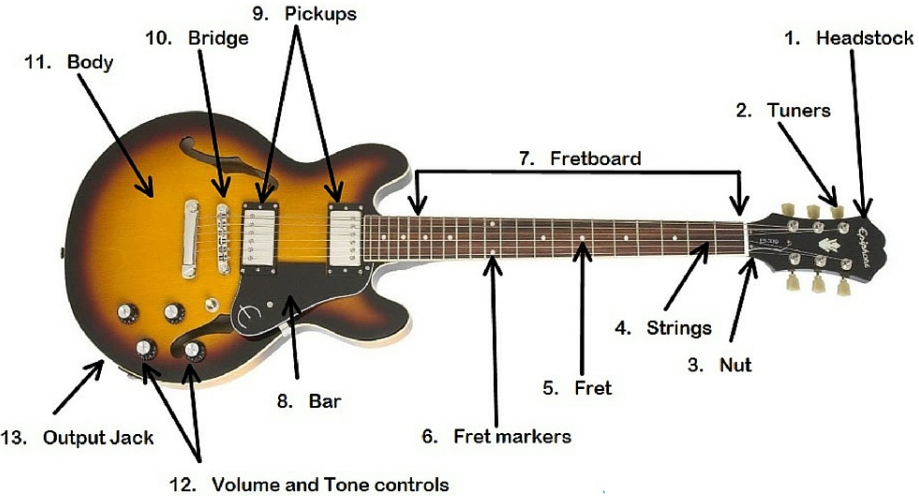
\includegraphics[width=0.9\textwidth]{guitar_parts.png}
		\caption{Illustration of an electric guitar and its parts \cite{coustii}.}
		\label{fig:guitar_parts}
\end{figure}

In the figure several parts are highlighted, but not all of them influence the sound, in the case where the guitar is not amplified. The pickups, the volume and the tone control have a large influence on the sound, when amplified, but they have no influence when not amplified. The tuners do have an influence on the sound, but more in the sense of making sure the guitar is in tune, which also is more or less the case with the fretboard. 
The parameters that will be investigated and have an influence on the sound, when not amplified, are:

\begin{itemize}
 \item String thickness and material
 \item String action
 \item Bridges
\end{itemize}

\subsection{String thickness and material}
String thickness (gauge) affects the sound of a guitar a lot. String gauge affects the tone of the sound and the sustain of the sound. Tone is a very broad term, which says something about how a string sounds. Often tone is described in subjective terms such as warm, deep, crunchy etc. \cite{premierguitar}. Sustain describes the period from when a tone is played until it fades out. Thicker strings will increase the sustain compared to thinner ones. Thicker strings will also increase the volume compared to thinner ones \cite{Helsinki}.
The material of the string also have an effect on its sound. Some of the materials used for electric guitar strings are: Nickel-plated steel, pure nickel and Stainless steel. Describing how the string material affects the sound is also often done in similar terms as for describing tone. E-Home Recording Studio fx. describes Nickel-plated steel as follows:
\\*
\\*
\textit{"Nickel-Plated Steel – which has a good combination of warmth and brightness, a strong picking attack, and is the most popular option."}\cite{E-Home}

\subsection{String action}
String action describes the distance from the strings to the fretboard on a guitar. A higher action allows the strings to vibrate more freely and thereby increasing the sustain of the tone \cite{sweetwater}. If the string action is set too low, distortion can occur when a note is tapped.  

\subsection{Bridges}
The bridge on an electric guitar is where the playable area of the guitar strings begins. The purpose of the bridge is to keep the strings fixed on the body, but without adding too much friction to the strings. This is because it is wanted to transfer as less string vibration to the bridge as possible. Two main categories of electrical guitar bridges exist; the fixed bridges and the moving bridges. The type of bridge has an effect on several aspects when playing the guitar, but it is the string-friction on the bridge that has the largest effect on the sound \cite{seymourduncan}.
\\*
\\*
Other physical parts on an electric guitar such as the fretboard, the nut and the body do have an effect on the non amplified sound, because some of the string vibration will be transferred to these parts. These parts are however parts that are difficult to change, without decreasing the quality set by the factory.   




